\section{Closed forms and light cones}\label{sec:closed}

\motiv{\vet{The path-sum bound of Chapter~\ref{sec:master} is exact bookkeeping: it counts the
sequences of terms that can carry a signal. To read it as a statement about distances, we
replace the count of paths by something that only sees pairs of sites, the \emph{site matrix},
whose entry at $(u,u')$ adds up the strengths of the terms containing both sites. A path of $k$
terms visits $k+1$ sites, one in the probe's region, one in each of the $k-1$ overlaps of
consecutive supports, and one in the observable's region; its weight is at most the product of
the matrix entries along those sites. Summing over all site sequences gives an entry of the
$k$-th power of the matrix, and summing the series gives its exponential.

From there the
published forms follow by three estimates: a decay function bounds the entries, a bounded
geometry bounds the row sums and makes distant entries of the powers vanish, and the tail of the
exponential series gives the light cone. \vetnew{A last section extends all of these to negative
times when the negated generators are contractive as well, as they are for a Hamiltonian.}}}

\subsection{The site matrix and walks}\label{subsec:sitematrix}

\vet{Throughout, $(S_i,L_i,\kappa_i)_{i\in I}$ is a family of local generators on a causal net
over an arbitrary set of sites $\Lambda$, and $T:=\bigcup_iS_i$ is the finite set of
\revs{\emph{touched sites}, the sites the family touches}. We write $\chi_i(u):=\ind{u\in S_i}$ for the indicator of a support.}

\begin{definition}[site matrix, walks]\label{def:sitematrix}
\vet{The \emph{site matrix} of the family is
\begin{equation}\label{eq:h}
  h_{uu'}:=\sum_{i\in I:\ u\in S_i,\ u'\in S_i}\kappa_i=\sum_i\kappa_i\,\chi_i(u)\,\chi_i(u')
  \qquad(u,u'\in\Lambda),
\end{equation}
so that $h_{uu}=\sum_{i\ni u}\kappa_i$. The \emph{walk weights} are defined by
$w_0(y,x):=\ind{y=x}$ and
\begin{equation}\label{eq:walk}
  w_{k+1}(y,x):=\sum_{z\in T}h_{yz}\,w_k(z,x).
\end{equation}
For a region $Y$, the \emph{boundary} $\bd Y:=Y\cap\bigcup_{i\in I^{\bd Y}}S_i$ is the set of
sites of $Y$ touched by a term crossing $Y$. For regions $Y,X$ put
\begin{equation}\label{eq:W}
  W_k(Y,X):=\sum_{y\in\bd Y}\ \sum_{x\in X\cap T}w_k(y,x).
\end{equation}}
\end{definition}

\vet{$w_k(y,x)$ is the total weight of the walks of $k$ steps from $y$ to $x$ through the
touched sites, each step $z\to z'$ weighted by $h_{zz'}$; on a finite lattice it is the entry
$(h^k)_{yx}$ (Proposition~\ref{prop:finite}). A walk may stay at a site, weighted by the diagonal
of $h$, or return to one. The boundary $\bd Y$ is the part of the probe's region that the
dynamics can reach from outside: a term inside $Y$ does nothing to an observable supported
outside $Y$ (Proposition~\ref{prop:annihilate}), so a signal enters $Y$ only through the sites
that a crossing term touches. Both $\bd Y$ and $X\cap T$ are finite, so $W_k$ is a finite sum.}

\needspace{10\baselineskip}
\begin{proposition}[properties]\label{prop:walkprops}
\vet{Let $K_1:=\sum_i\kappa_i|S_i|$.
\begin{enumerate}[label=(\alph*),nosep]
\item $h_{uu'}\ge0$, $h_{uu'}=h_{u'u}$, and $h_{uu'}=0$ unless $u,u'\in T$;
\item \vetnew{$\sum_{u'\in T}h_{uu'}\le K_1$ for every site $u$};
\item $w_k(y,x)\ge0$; for $k\ge1$, $w_k(y,x)=0$ unless $y,x\in T$, and $w_1(y,x)=h_{yx}$;
\item $\sum_{x\in T}w_k(y,x)\le q^k$ whenever every row sum $\sum_{u'\in T}h_{uu'}$ is at most
  $q\ge0$; hence $W_k(Y,X)\le|\bd Y|\,q^k$, and in particular $W_k(Y,X)\le|\bd Y|\,K_1^{\,k}$.
\end{enumerate}}
\end{proposition}

\begin{proof}
\vet{\begin{enumerate}[label=(\alph*),nosep]
\item Read off the definitions.
\item Exchanging the sums, $\sum_{u'\in T}\sum_{i:\,u,u'\in S_i}\kappa_i=\sum_{i\ni u}\kappa_i|S_i|\vetnew{{}\le K_1}$.
\item Read off the definitions.
\item By induction on $k$: for $k=0$ the sum is $\ind{y\in T}\le1$, and
$\sum_xw_{k+1}(y,x)=\sum_zh_{yz}\sum_xw_k(z,x)\le q^k\sum_zh_{yz}\le q^{k+1}$.\qedhere
\end{enumerate}}
\end{proof}

\vetnew{The proof of (b) gives the row sum exactly: $\sum_{u'\in T}h_{uu'}=\sum_{i\ni u}\kappa_i|S_i|$,
the total weighted size of the supports that contain $u$.}

\begin{figure}[t]
\centering
% Figure: a path of three terms from Y to X and a sequence of sites along it. Transcription (for
% cheap agents): seven sites 0..6 on a line; the probe's region Y = {0, 1} (left box), the
% observable's region X = {5, 6} (right box); three supports drawn as rounded boxes above the
% line: S_{i_1} = {1, 2, 3}, S_{i_2} = {3, 4}, S_{i_3} = {4, 5}; the chosen sites u_0 = 1 (in
% S_{i_1} ∩ Y, on the boundary of Y), u_1 = 3 (in S_{i_1} ∩ S_{i_2}), u_2 = 4 (in S_{i_2} ∩ S_{i_3}),
% u_3 = 5 (in S_{i_3} ∩ X), marked by filled circles and joined by arrows labelled h_{13}, h_{34},
% h_{45}; the weights κ_{i_1} ≤ h_{13}, κ_{i_2} ≤ h_{34}, κ_{i_3} ≤ h_{45} written under the arrows.
% The label S_{i_3} sits above the box S_{i_3}, clear of the box S_{i_2}; the label u_3 sits
% slightly to the right of site 5, above the box of X, clear of S_{i_3}.
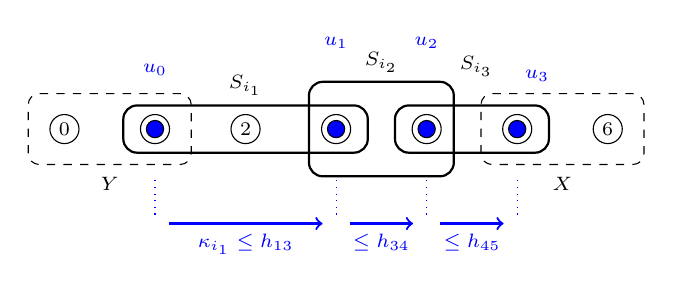
\begin{tikzpicture}[x=1.15cm,y=1cm,
  site/.style={circle,draw,fill=white,inner sep=1.6pt,font=\scriptsize},
  chosen/.style={circle,draw,fill=Blue,inner sep=2.2pt},
  edge/.style={rounded corners=5pt,draw,thick,fill=none},
  region/.style={rounded corners=4pt,draw,dashed,fill=none},
  lab/.style={font=\scriptsize}]
  % regions
  \draw[region] (-0.4,-0.45) rectangle (1.4,0.45);
  \node[lab] at (0.5,-0.7) {$Y$};
  \draw[region] (4.6,-0.45) rectangle (6.4,0.45);
  \node[lab] at (5.5,-0.7) {$X$};
  % supports
  \draw[edge] (0.65,-0.3) rectangle (3.35,0.3);   \node[lab] at (2,0.55) {$S_{i_1}$};
  \draw[edge] (2.7,-0.6) rectangle (4.3,0.6);     \node[lab] at (3.5,0.85) {$S_{i_2}$};
  \draw[edge] (3.65,-0.3) rectangle (5.35,0.3);   \node[lab] at (4.55,0.8) {$S_{i_3}$};
  % sites
  \foreach \s in {0,...,6} { \node[site] (s\s) at (\s,0) {\s}; }
  \node[chosen] at (1,0) {}; \node[chosen] at (3,0) {}; \node[chosen] at (4,0) {};
  \node[chosen] at (5,0) {};
  \node[lab,Blue] at (1,0.75) {$u_0$};
  \node[lab,Blue] at (3,1.1) {$u_1$};
  \node[lab,Blue] at (4,1.1) {$u_2$};
  \node[lab,Blue] at (5.22,0.68) {$u_3$};
  % the walk
  \draw[->,Blue,thick] (1.15,-1.2) -- (2.85,-1.2) node[midway,below,lab,Blue] {$\kappa_{i_1}\le h_{13}$};
  \draw[->,Blue,thick] (3.15,-1.2) -- (3.85,-1.2) node[midway,below,lab,Blue] {$\le h_{34}$};
  \draw[->,Blue,thick] (4.15,-1.2) -- (4.85,-1.2) node[midway,below,lab,Blue] {$\le h_{45}$};
  \foreach \s in {1,3,4,5} { \draw[Blue,dotted,thin] (\s,-0.65) -- (\s,-1.1); }
\end{tikzpicture}

\caption{\vet{A path of three terms from the probe's region $Y$ to the observable's region $X$,
and a sequence of sites along it: $u_0\in S_{i_1}\cap Y$ lies on the boundary $\bd Y$, each
$u_j$ in the overlap $S_{i_j}\cap S_{i_{j+1}}$, and $u_3\in S_{i_3}\cap X$. Each step
$u_{j-1}\to u_j$ stays inside the support $S_{i_j}$, so $\kappa_{i_j}\le h_{u_{j-1}u_j}$: the
weight of the path is at most the weight of this walk. Theorem~\ref{thm:domination} makes the
idea precise without choosing the sites, by expanding the walk sum through the indicators of
the supports.}}
\label{fig:walkchoice}
\end{figure}

\begin{theorem}[domination of the path count]\label{thm:domination}
\vet{For every $k\ge1$ and all regions $X,Y$,
\begin{equation}\label{eq:domination}
  P_k(Y,X)\le W_k(Y,X).
\end{equation}}
\end{theorem}

\begin{proof}
\vet{Induction on $k$, the claim quantified over all $Y$.

\emph{$k=1$.} $P_1(Y,X)$ is the sum of $\kappa_i$ over the terms crossing $Y$ and meeting $X$.
Expanding \eqref{eq:W} with $w_1=h$ and \eqref{eq:h},
\[
  W_1(Y,X)=\sum_i\kappa_i\Bigl(\sum_{y\in\bd Y}\chi_i(y)\Bigr)\Bigl(\sum_{x\in X\cap T}\chi_i(x)\Bigr).
\]
For a term $i$ crossing $Y$ and meeting $X$, some site of $S_i$ lies in $Y$, hence in $\bd Y$,
and some site of $S_i$ lies in $X$, hence in $X\cap T$; so both brackets are at least $1$.
Every other term contributes a nonnegative amount. Hence $P_1\le W_1$.

\emph{Step, the left side.} The recursion of Proposition~\ref{prop:pathcount} gives
$P_{k+1}(Y,X)=\sum_{i\in Q}\kappa_iP_k(S_i,X)$, with $Q$ the terms crossing $Y$ and missing $X$.
\vetnew{We extend the notation: $w_k(z,X):=\sum_{x\in X\cap T}w_k(z,x)\ge0$. By the induction
hypothesis for the region $S_i$, and since $\bd S_i\subseteq S_i$,
$P_k(S_i,X)\le W_k(S_i,X)\le\sum_{z\in S_i}w_k(z,X)$.}

\emph{Step, the right side.} Expanding \eqref{eq:W} with \eqref{eq:walk} and \eqref{eq:h}, and
summing over $z$ first,
\[
  W_{k+1}(Y,X)=\sum_i\kappa_i\Bigl(\sum_{y\in\bd Y}\chi_i(y)\Bigr)\sum_{z\in S_i}\vetnew{w_k(z,X)}.
\]

\emph{Comparison.} For $i\in Q$ the bracket is at least $1$, as in the base case, and every
other term is nonnegative. So
$P_{k+1}(Y,X)\le\sum_{i\in Q}\kappa_i\sum_{z\in S_i}\vetnew{w_k(z,X)}\le W_{k+1}(Y,X)$.}
\end{proof}

\vet{What the domination loses: a walk may return to a site it has visited, while a path never
repeats a term immediately, and a walk continues after reaching $X$, while a path stops. Both
effects are visible in Example~\ref{ex:chainwalk}, where equality holds at $k=2$ and the walk
weights are strictly larger from $k=3$ on.}

\subsection{The walk series and the matrix exponential}

\begin{theorem}[closed form (i): the walk series]\label{thm:walkseries}
\vet{Let the net be causal, $t\ge0$, $a\in\cA(X)$ and $b\in\cA(Y)$. Then
\begin{equation}\label{eq:walkseries}
  \norm{\comm{A(t)}b}\le2\norm a\norm b\Bigl(\ind{X\cap Y\ne\emptyset}
  +\sum_{k\ge1}\frac{(2t)^k}{k!}\,W_k(Y,X)\Bigr),
\end{equation}
the series converging with sum at most $|\bd Y|\,(e^{2K_1t}-1)$.}
\end{theorem}

\begin{proof}
\vet{Termwise, $(2t)^kP_k/k!\le(2t)^kW_k/k!\le|\bd Y|(2tK_1)^k/k!$ by Theorem~\ref{thm:domination}
and Proposition~\ref{prop:walkprops}(d); so the walk series converges by comparison with the
exponential series, and \eqref{eq:master} gives \eqref{eq:walkseries}.}
\end{proof}

\vetnew{The terms of this series are the \emph{walk terms}: for the pair $(Y,X)$ and $k\ge0$,
\begin{equation}\label{eq:walkterms}
  \omega_k(t):=\frac{(2t)^{k+1}}{(k+1)!}\,W_{k+1}(Y,X)=\gamma_k(t)\,W_{k+1}(Y,X),
\end{equation}
with the coefficient $\gamma_k$ of \eqref{eq:truncbound}, so that the series in
\eqref{eq:walkseries} is $\sum_{k\ge0}\omega_k(t)$. We shift the index by one so that
$\omega_k$ carries the walks of $k+1$ steps as $\gamma_k$ carries the paths of length $k+1$. The
walk terms depend on the strengths $\kappa_i$, through the site matrix in $W_{k+1}$, and on the
pair $(Y,X)$; Chapter~\ref{sec:approx} uses them.}

\begin{proposition}[finite lattice]\label{prop:finite}
\vet{Let $\Lambda$ be finite and regard $h$ as a matrix. Then $w_k(y,x)=(h^k)_{yx}$, and for
$s\in\R$ the entries of the matrix exponential are the series of the entries of the powers,
$(e^{sh})_{yx}=\sum_{n\ge0}s^n(h^n)_{yx}/n!$. Consequently
\begin{equation}\label{eq:matrixform}
  \norm{\comm{A(t)}b}\le2\norm a\norm b\Bigl(\ind{X\cap Y\ne\emptyset}
  +\sum_{y\in\bd Y}\sum_{x\in X\vetnew{{}\cap T}}\bigl(e^{2th}-1\bigr)_{yx}\Bigr).
\end{equation}}
\end{proposition}

\begin{proof}
\vet{$w_{k+1}(y,x)=\sum_{z\in T}h_{yz}(h^k)_{zx}=\sum_{z\in\Lambda}h_{yz}(h^k)_{zx}$, the terms
with $z\notin T$ vanishing, which is $(h^{k+1})_{yx}$. The exponential series converges in any
algebra norm on the matrices, and every entry is bounded by the norm, so the entries converge to
the entries. Then \eqref{eq:matrixform} is \eqref{eq:walkseries} with the series summed
entrywise\vetnew{, over the pairs of $\bd Y\times(X\cap T)$ as in \eqref{eq:W}}.}
\end{proof}

\vetnew{The inner sum in \eqref{eq:matrixform} may equally run over all of $X$: for $x\notin T$
the column $x$ of $h$ vanishes, so $(h^n)_{yx}=0$ for $n\ge1$ and the entry
$(e^{2th}-1)_{yx}$ is zero.}

\vet{Inequality \eqref{eq:matrixform} is the matrix form of the Lieb-Robinson bound in
\cite{chen-lucas-yin}, with the sum over the probe's region sharpened to its boundary.}

\begin{example}[the three-qubit chain, continued]\label{ex:chainwalk}
\vet{For $H=\sigma^z_0\sigma^z_1+\tfrac12\sigma^x_1\sigma^x_2$ of Example~\ref{ex:chain}, with
$S_1=\{0,1\}$, $\kappa_1=1$, $S_2=\{1,2\}$, $\kappa_2=\tfrac12$, $X=\{0\}$ and $Y=\{2\}$:
$T=\{0,1,2\}$, $\bd Y=\{2\}$, and
\[
  h=\begin{pmatrix}1&1&0\\[2pt] 1&\tfrac32&\tfrac12\\[2pt] 0&\tfrac12&\tfrac12\end{pmatrix}.
\]
The walk weights from the boundary site $2$ to the observable's site $0$ follow from
\eqref{eq:walk}: $w_1(2,0)=h_{20}=0$; $w_2(2,0)=h_{21}w_1(1,0)+h_{22}w_1(2,0)=\tfrac12$; and,
with $w_2(1,0)=h_{10}w_1(0,0)+h_{11}w_1(1,0)+h_{12}w_1(2,0)=1+\tfrac32=\tfrac52$,
$w_3(2,0)=h_{21}w_2(1,0)+h_{22}w_2(2,0)=\tfrac54+\tfrac14=\tfrac32$. The path counts are
$P_2=\tfrac12$ and $P_k=0$ otherwise: equality at $k=2$, and from $k=3$ on the walks revisit
sites while the paths have stopped. The path series is exactly $2t^2$; the walk series
\eqref{eq:walkseries} is $2\bigl(\tfrac{(2t)^2}{2!}\cdot\tfrac12+\tfrac{(2t)^3}{3!}\cdot\tfrac32
+\dots\bigr)=2t^2+4t^3+\dots=2\bigl(e^{2th}-1\bigr)_{20}$.}
\end{example}

\subsection{Decay functions}

\vet{\vetnew{A decay function is a function of pairs of sites that reproduces itself under convolution;
the bounds use a constant multiple of it that dominates the site matrix.}}

\begin{definition}[decay function]\label{def:kernel}
\vet{A \vetnew{\emph{decay function}} is a function $F:\Lambda\times\Lambda\to[0,\infty)$ with a constant
$C_F>0$ such that for all $x,y$ and every finite $T'\subseteq\Lambda$,
\begin{equation}\label{eq:reproducing}
  \sum_{z\in T'}F(x,z)\,F(z,y)\le C_F\,F(x,y).
\end{equation}
An \emph{$F$-bound} of the family is a number $N_F\ge0$ with $h_{xy}\le N_FF(x,y)$ for all
$x,y$. Write $\Sigma_F(Y,X):=\sum_{y\in\bd Y}\sum_{x\in X\cap T}F(y,x)$.}
\end{definition}

\begin{example}[a decay function on the chain]\label{ex:kernel}
\vet{On a finite chain $\Lambda=\{0,\dots,n\}$ with $d(x,y)=|x-y|$ and nearest-neighbour terms
(the constants below do not depend on $n$), \vetnew{the function $F(x,y)=e^{-\lambda|x-y|}$ with
$\lambda>0$ is not enough}: $\sum_zF(x,z)F(z,y)$ counts the $|x-y|+1$ sites between $x$
and $y$ with the full weight $e^{-\lambda|x-y|}$, so no constant $C_F$ works uniformly in $n$.

The standard remedy is a polynomial factor, $F(x,y)=e^{-\lambda|x-y|}/(1+|x-y|)^2$: the exponentials obey
$e^{-\lambda(|x-z|+|z-y|)}\le e^{-\lambda|x-y|}$, \vetnew{and with $m=y-x$ and $j=z-x$,
$(1+|j|)(1+|m-j|)\ge\tfrac12(1+|m|)(1+\min\{|j|,|m-j|\})$, so
$\sum_zF(x,z)F(z,y)\le C_F\,F(x,y)$ with
$C_F=\sup_m\sum_{j\in\mathbb Z}4/(1+\min\{|j|,|m-j|\})^2<\infty$,
uniformly in $m$} (the constant can be sharpened). For the nearest-neighbour family with all
$\kappa_i=1$, the least
$F$-bound is $N_F=4e^{\lambda}$: the diagonal needs $h_{xx}=2\le N_F$ and a neighbouring pair
needs $h_{x,x+1}=1\le N_Fe^{-\lambda}/4$.}
\end{example}

\vet{In general, for \vetnew{a distance $d$ (Definition~\ref{def:geometry})} and a non-increasing
$F_0:[0,\infty)\to(0,\infty)$, the \vetnew{function} $F(x,y)=F_0(d(x,y))$ satisfies \eqref{eq:reproducing} as soon as the reproducing constant
$C_F=\sup_{x,y}\sum_zF_0(d(x,z))F_0(d(z,y))/F_0(d(x,y))$ is finite, which is an assumption on
$F_0$ and the lattice; for the lattice $\mathbb Z^\nu$ Chapter~\ref{sec:qudit} quotes the
constant from the literature and computes it on finite pieces.
\vetnew{The least $F$-bound is then the literature's $F$-norm of the interaction, when each
support carries one term (Chapter~\ref{sec:qudit}); every larger number is an $F$-bound as
well.}}

\begin{theorem}[closed form (ii): decay functions]\label{thm:decay}
\vet{Under the hypotheses of Theorem~\ref{thm:walkseries}, for a \vetnew{decay function} $F$ with constant
$C_F$ and an $F$-bound $N_F$,
\begin{equation}\label{eq:decayform}
  \norm{\comm{A(t)}b}\le2\norm a\norm b\Bigl(\ind{X\cap Y\ne\emptyset}
  +\frac{e^{2N_FC_Ft}-1}{C_F}\,\Sigma_F(Y,X)\Bigr).
\end{equation}}
\end{theorem}

\begin{proof}
\vet{By induction on $k$, $w_k(y,x)\le N_F^{\,k}C_F^{\,k-1}F(y,x)$ for $k\ge1$: the case $k=1$ is
$h\le N_FF$, and the step is
$w_{k+1}(y,x)=\sum_{z\in T}h_{yz}w_k(z,x)\le N_F^{\,k+1}C_F^{\,k-1}\sum_{z\in T}F(y,z)F(z,x)
\le N_F^{\,k+1}C_F^{\,k}F(y,x)$ by \eqref{eq:reproducing}. Summing over $\bd Y$ and $X\cap T$,
$W_k(Y,X)\le N_F^{\,k}C_F^{\,k-1}\Sigma_F(Y,X)$, and the series in \eqref{eq:walkseries} is at
most $(\Sigma_F/C_F)\sum_{k\ge1}(2N_FC_Ft)^k/k!$.}
\end{proof}

\vet{With $F(x,y)=F_0(d(x,y))$, inequality \eqref{eq:decayform} is the decay-function form of
\cite{nsy2019}. Their form offers a second option, the sum over the boundary of the
observable's region instead of the probe's: it is the same statement with the roles of the two
observables exchanged, which for a group of automorphisms follows from
\vetnew{the identity $\norm{\comm{\tau_t(A)}B}=\norm{\comm{A}{\tau_{-t}(B)}}$ of
Theorem~\ref{thm:exchange} (Chapter~\ref{sec:qudit}), with Theorem~\ref{thm:reverse} for the
negative time}.}

\subsection{Bounded geometry and light cones}\label{subsec:geometry}

\begin{definition}[bounded geometry]\label{def:geometry}
\vet{Let $d:\Lambda\times\Lambda\to\R$ satisfy $d(u,u)=0$ and $d(u,u'')\le d(u,u')+d(u',u'')$.
The family has \emph{bounded geometry} $(g,\ell,p,\rho)$ if every site lies in the supports of at
most $g$ indices $i$, every $\kappa_i\le\ell$, every $|S_i|\le p$, and $d(u,u')\le\rho$ for $u,u'$
in a common support ($\ell,\rho\ge0$). Write $v:=2g\ell p$.}
\end{definition}

\vetnew{We call a function $d$ with $d(u,u)=0$ and the triangle inequality a \emph{distance}.
It is not assumed symmetric, so $d(u,u')$ and $d(u',u)$ may differ, and we keep the order of the
arguments throughout: the first on the probe's side, the second on the observable's.}

\begin{proposition}[walks and distance]\label{prop:distance}
\vet{With bounded geometry $(g,\ell,p,\rho)$:
\begin{enumerate}[label=(\alph*),nosep]
\item $w_k(y,x)=0$ whenever $k\rho<d(y,x)$;
\item every row sum of $h$ is at most $g\ell p$, so $W_k(Y,X)\le|\bd Y|\,(g\ell p)^k$.
\end{enumerate}}
\end{proposition}

\begin{proof}
\vet{\begin{enumerate}[label=(\alph*),nosep]
\item By induction: a nonzero term $h_{yz}w_k(z,x)$ of \eqref{eq:walk} has $y,z$ in a common
support, so $d(y,z)\le\rho$, and $d(z,x)\le k\rho$; the triangle inequality gives
$d(y,x)\le(k+1)\rho$.
\item \vetnew{The row sum at $u$ is $\sum_{i\ni u}\kappa_i|S_i|$ (the paragraph after
Proposition~\ref{prop:walkprops}), a sum of} at most $g$
terms, each at most $\ell p$.\qedhere
\end{enumerate}}
\end{proof}

\begin{lemma}[tail of the exponential series]\label{lem:tail}
\vet{For $x\ge0$ and $r\in\N$: $\sum_{k\ge r}x^k/k!\le(x^r/r!)\,e^x$, since
$x^{r+j}/(r+j)!\le(x^r/r!)(x^j/j!)$ by $r!\,j!\le(r+j)!$.}
\end{lemma}

\begin{theorem}[closed form (iii): bounded geometry]\label{thm:geometry}
\vet{Under the hypotheses of Theorem~\ref{thm:walkseries} and bounded geometry $(g,\ell,p,\rho)$,
let $r\ge1$ satisfy $(r-1)\rho<d(y,x)$ for all $y\in\bd Y$, $x\in X\cap T$. Then
\begin{equation}\label{eq:geometryform}
  \norm{\comm{A(t)}b}\le2\norm a\norm b\Bigl(\ind{X\cap Y\ne\emptyset}
  +|\bd Y|\,\frac{(vt)^r}{r!}\,e^{vt}\Bigr),\qquad v=2g\ell p .
\end{equation}}
\end{theorem}

\begin{proof}
\vet{For $k<r$ every pair in \eqref{eq:W} is farther than $k\rho$, so $W_k(Y,X)=0$ by
Proposition~\ref{prop:distance}(a); for $k\ge r$, $W_k\le|\bd Y|(g\ell p)^k$ by (b). The series in
\eqref{eq:walkseries} is therefore at most $|\bd Y|\sum_{k\ge r}(vt)^k/k!$, and
Lemma~\ref{lem:tail} applies.}
\end{proof}

\begin{figure}[t]
\centering
% Figure: the light cone of the exponential form. Transcription (for cheap agents): axes, time t
% to the right and the distance d(∂Y, X ∩ T) of Chapter 3 upward; a straight line d = c t from
% the origin (the cone's edge, c = ρ(1 + e^μ) v / μ, written at the right end of the line); the
% region above the line, up to the top of the drawing, is shaded and labelled, in its upper left
% corner, "bound ≲ e^{-μ d/ρ + (1+e^μ) v t}, exponentially small"; the region below the line is
% labelled "bound trivial (at most 2‖a‖‖b‖)"; near the right edge of the shading a point above the
% line with a dashed vertical segment down to the line; outside the shading, to the right of the
% point and above the cone's label, "decay rate μ/ρ in the distance to the cone (dashed)". No label
% touches the line or the dashed segment.
\begin{tikzpicture}[x=1cm,y=1cm,>={Stealth[length=5pt]}]
  \fill[Blue!8] (0,0) -- (5.2,2.6) -- (5.2,3.75) -- (0,3.75) -- cycle;
  \draw[->] (0,0) -- (5.8,0) node[right,font=\small] {$t$};
  \draw[->] (0,0) -- (0,3.9) node[above,font=\small] {$\dist(\bd Y,X\cap T)$};
  \draw[Blue,thick] (0,0) -- (5.2,2.6);
  \node[font=\scriptsize,Blue,anchor=west] at (5.3,2.6) {$\dist=\rho\,\dfrac{(1+e^{\mu})v}{\mu}\,t$};
  \node[font=\scriptsize,align=left,anchor=west] at (0.15,3.15)
    {bound $\lesssim e^{-\mu\dist/\rho+(1+e^{\mu})vt}$,\\ exponentially small};
  \node[font=\scriptsize,align=center] at (4.0,0.75) {bound trivial\\ ($\le2\norm a\norm b$)};
  \fill (4.5,3.35) circle (1.6pt);
  \draw[dashed] (4.5,3.35) -- (4.5,2.25);
  \node[font=\scriptsize,align=left,anchor=west] at (5.3,3.45)
    {decay rate $\mu/\rho$ in the\\ distance to the cone (dashed)};
\end{tikzpicture}

\caption{\vet{The light cone of Theorem~\ref{thm:cone}, for $\mu,\rho>0$: in the plane of the
distance between the probe's boundary and the observable's region against the time $t$, the
bound is at most a constant times $e^{-\mu\,\dist/\rho+(1+e^{\mu})vt}$, so it is small outside
the cone $\dist>\rho(1+e^{\mu})vt/\mu$ (shaded) and trivial inside it. The slope of the line is
schematic. The velocity $(1+e^{\mu})v\rho/\mu$ and the decay rate $\mu/\rho$ are those of the
bound, not of the dynamics.}}
\label{fig:lightcone}
\end{figure}

\begin{theorem}[closed form (iv): the exponential light cone]\label{thm:cone}
\vet{Under the hypotheses of Theorem~\ref{thm:geometry}, for every real $\mu$,
\begin{equation}\label{eq:coneform}
  \norm{\comm{A(t)}b}\le2\norm a\norm b\Bigl(\ind{X\cap Y\ne\emptyset}
  +|\bd Y|\,e^{vt}\,e^{-\mu r}\bigl(e^{e^{\mu}vt}-1\bigr)\Bigr).
\end{equation}}
\end{theorem}

\begin{proof}
\vet{For $r\ge1$ and $x\ge0$, $x^r/r!=e^{-\mu r}(e^{\mu}x)^r/r!\le e^{-\mu r}\sum_{j\ge1}(e^{\mu}x)^j/j!
=e^{-\mu r}(e^{e^{\mu}x}-1)$; insert $x=vt$ into \eqref{eq:geometryform}.}
\end{proof}

\vet{Take $\mu,\rho>0$, regions with $\bd Y$ and $X\cap T$ nonempty, and let
\vetnew{$\dist(\bd Y,X\cap T)$}$:=\min\{d(y,x):y\in\bd Y,\ x\in X\cap T\}$ be positive; put
$r=\lceil\vetnew{\dist(\bd Y,X\cap T)}/\rho\rceil\ge1$. The hypothesis of Theorem~\ref{thm:geometry}
holds, and \eqref{eq:coneform}
is at most a constant times $e^{-\mu\,\vetnew{\dist(\bd Y,X\cap T)}/\rho+(1+e^{\mu})vt}$: a light cone of
velocity $(1+e^{\mu})v\rho/\mu$ with decay rate $\mu/\rho$ outside it
(Figure~\ref{fig:lightcone}).}

\begin{example}[a nearest-neighbour chain]\label{ex:cone}
\vet{Nearest-neighbour terms on the chain $\{0,\dots,n\}$, one term $\{j,j+1\}$ per bond with
$\kappa_j\le\ell$: each site lies in at most $g=2$ supports of size $p=2$ and diameter
$\rho=1$, so $v=8\ell$. For an observable at the site $0$ and a probe at the site $n\ge1$, the
boundary is $\bd Y=\{n\}$ and $r=n$, and Theorem~\ref{thm:geometry} reads
$\norm{\comm{A(t)}b}\le2\norm a\norm b\,(8\ell t)^ne^{8\ell t}/n!$. With $\mu=1$,
Theorem~\ref{thm:cone} gives a light cone of velocity $(1+e)\cdot8\ell\approx30\ell$ and decay
rate $1$ per site outside it. The velocity is an artefact of the walk bound; on the three-site
chain of Example~\ref{ex:chain} the path series itself is sharp to leading order at short
times.}
\end{example}

\subsection{Time reversal}\label{subsec:reversal}

\vet{We proved the path-sum bound for $t\ge0$, because hypothesis (G3) is a statement about
$e^{tL_J}$ for $t\ge0$. If the family also satisfies (G3) with every $L_i$ replaced by $-L_i$,
which is the case for a group of automorphisms, \revs{we say that the family has a
\emph{contractive negation}, and then} the bound holds for all times.}

\begin{theorem}[time reversal]\label{thm:reverse}
\vet{Let the net be causal, and suppose $\norm{e^{-tL_J}}\le1$ for every $J\subseteq I$ and
$t\ge0$. Then \eqref{eq:master}, \eqref{eq:walkseries} and \eqref{eq:decayform} hold for every
$t\in\R$ with $|t|$ in place of \vetnew{$t$.}}
\end{theorem}

\begin{proof}
\vet{The negated family $(S_i,-L_i,\kappa_i)$ satisfies (G1) and (G2), since
$\norm{-L_ic}=\norm{L_ic}$ and $\cA(Z\cup S_i)$ is a subspace, and (G3) by hypothesis; it has the
same supports and strengths, hence the same paths, counts, site matrix and walk weights, and its
dynamics at time $|t|$ is $e^{|t|(-L)}=e^{tL}$ for $t<0$. Apply the bounds to it.}
\end{proof}

\vetnew{The matrix form \eqref{eq:matrixform} and the bounded-geometry and light-cone forms
\eqref{eq:geometryform} and \eqref{eq:coneform} follow from \eqref{eq:walkseries} alone, by the
proofs of Proposition~\ref{prop:finite} and Theorems~\ref{thm:geometry} and~\ref{thm:cone}.
Applied to the negated family, which has the same supports and strengths, they too hold for every
$t\in\R$ with $|t|$ in place of $t$ under the hypothesis of Theorem~\ref{thm:reverse}.}

\subsection*{Notes and references}
\vet{\emph{Site matrix.} The review \cite{chen-lucas-yin} defines $h_{uu'}$ for two-site terms,
with $\norm{H_{uu'}}$ off the diagonal and the sum of the strengths at a site on it (its
eq.~(3.35)); \cite{chen-lucas2021} writes $h_{ij}=\sum_{X\ni i,j}\norm{H_X}$ for general
supports. Definition~\ref{def:sitematrix} is the latter with $\kappa_i$ in place of $\norm{H_X}$,
and \eqref{eq:matrixform} is \vetnew{the review's (3.36), with its constant doubled and the $-1$
that the series proof gives}; the review's commutator quantity is half of $C_{X,Y}(t)$.

\emph{Boundary and decay functions.} The boundary $\bd Y$ is the $\Phi$-boundary of
\cite{nsy2019}, eq.~(3.20). Decay functions $F_0$ with a reproducing constant and the $F$-norm
are \cite{nsy2019}, eqs.~(3.8)--(3.9) and (3.14); \vetnew{Theorem~3.1 of \cite{nsy2019}} is \eqref{eq:decayform}
with $F=F_0\circ d$ and $N_F$ the $F$-norm, the exponent $2N_FC_Ft$ being their $2I_{t,s}$ for a
time-independent interaction. Only the finite-sum form \eqref{eq:reproducing} enters here, so
neither a metric nor the convergence of $\sum_yF_0(d(x,y))$ is needed before
Chapter~\ref{sec:qudit}.

\emph{Geometry.} The bounded-degree form is the review's Proposition~3.5, whose constants
($4(g-1)h$ for the velocity and $K=1/(1-2/e)$ for the tail) are sharper than
\eqref{eq:geometryform}'s $v=2g\ell p$ and $e^{vt}$, because the review's walks never return
along the edge they came from; the exponential form is \vetnew{the review's Example~3.6}.}

\paragraph{Checks.} {\small The site matrix, walk weights and series of
Example~\ref{ex:chainwalk}, the domination on random hypergraphs, the constants $C_F$ (the least
constant on a chain of $40$ sites at $\lambda=\tfrac12$ is $3.72$) and $N_F=4e^{\lambda}$ of
Example~\ref{ex:kernel}, the vanishing of $(h^k)_{xy}$ below the distance, the tail bound behind
Example~\ref{ex:cone} and the comparison with the review's Proposition~3.5 are computed by
\texttt{checks/m1b\_check.py}.}
